\chapter{アプローチ}
\label{chap:approach}

\ref{section:purpose}で,本研究の目的を,
動作中のコンピュータのメモリのダンプをリアルタイムで解析することで,コンピュータの状態をリモートホストから知ることができるようにする,と定義した.

そこで本章では,メモリのダンプをリアルタイムで取得.解析する上で前提となる情報と,この手法における課題について述べる.

\section{オペレーティングシステムのコンテキスト}
\label{section:context}

コンピュータの状態,すなわちオペレーティングシステムの動作中におけるコンピュータのコンテキストは,コンピュータ内部におけるレジスタの値および,内部から参照できる仮想アドレス空間上に保持されている.
その例を下に示す.

あるプロセスを実行する際に,プロセッサはインストラクションポインタレジスタの命令を読み込み,逐次実行をしていく.
call命令などで別の関数を呼ぶ際には,その時点におけるインストラクションポインタレジスタの値をメモリ上に退避し,関数が終わった際に,呼び出し元に返るように設定されている.
実行コードが整合性を保っているかは,実行可能ファイルを生成したコンパイラの責務なので,本論文では述べないが,
プロセッサはプログラムの実行を行う際,レジスタの値を参照,退避,復帰,上書きさせることで,状態を保持,進行させていると言える.

プロセッサがレジスタの値を参照しそれを仕組みは,カーネルのコードを実行する際にも言える.
ここでは,オペレーティングシステムから見たコンピュータの状態として,プロセスの切り替え処理,コンテキストスイッチにおける処理の流れを述べる.
コンテキストスイッチとは,割り込み処理などによって定期的に呼ばれるプロセススケジューラーから呼ばれる機構である.
この機構は,実行中のプロセスの状態,すなわち,各レジスタの値および仮想アドレス空間に関する情報などをカーネルが管理しているメモリ上にあるデータ構造の中に退避する.

本セクションのまとめとして,コンピュータの状態は,ある瞬間においてはレジスタの値であり,この状態を保存する際は,メモリ上にレジスタの値を退避させていることを述べた.

\subsection{task\_struct構造体}

\ref{section:context}でコンテキストスイッチにおいて,退避されるプロセスの情報は,対応したデータ構造に退避されると述べたが,この時に使用されるデータ構造がtask\_struct構造体である.
task\_struct構造体には,一つのプロセスの情報の全て(?)が格納されている.その中には,仮想アドレス空間に関する情報を保持するmm\_struct構造体を参照するフィールドも存在する.

コンテキストスイッチ時には,task\_struct構造体に保持されている情報をレジスタに復帰させることで,中断される直前の情報を復元している.

\subsection{オペレーティングシステムのビルドにおけるコンフィグ}

task\_struct構造体をはじめとして,Linuxカーネルの変数や型,関数は,様々なアーキテクチャやカーネルコンフィグに対応するため,マクロによって分岐されている.
この分岐が確定するのは,Linuxカーネルをビルドするときであり,構造体のメンバへのアクセス,関数のアドレスなどはコンパイラが保証している.

実際のカーネルのバイナリは,vmlinuxとしてコンパイルされた後,stripされbzImageとなる.
ユーザーが作成したカーネルモジュールなどで関数を呼び出す際は,シンボルとアドレスの変換表である`/boot/System.map`を参照し,仮想アドレスを得たのち,
実際にメモリにアクセスする際に物理メモリアドレスを算出しアクセスしている.

\subsection{ホスト自身によるレジスタやシンボルの参照}

\ref{section:context}で述べたように,オペレーティングシステムでは,その実行中のコンテキストにおいて,
レジスタの値などを退避する際,そのプロセッサ自身が'push'命令などを用いてメモリにアクセスできる.

さらにレジスタを参照して,Memory Management Unitを通じ,ページウォークなどをすることも可能となっている.

本研究では,メモリの情報のみから監視対象ホストのオペレーティングシステムのコンテキストを復元することを試みるが,
CPUレジスタの値は直接知ることができないため,例えばプロセスの一覧を取得したい場合は,コンテキストスイッチ時に退避された値を辿っていく必要がある.
しかし,上述の通りtask\_structはビルドされた際のカーネルコンフィグによって,どのフィールドが先頭アドレスからどのオフセットに保持されているかは変動する.

\begin{figure}[htbp]
    \caption{Linuxにおけるmmu}
    \label{fig:mmu}
    \begin{center}
        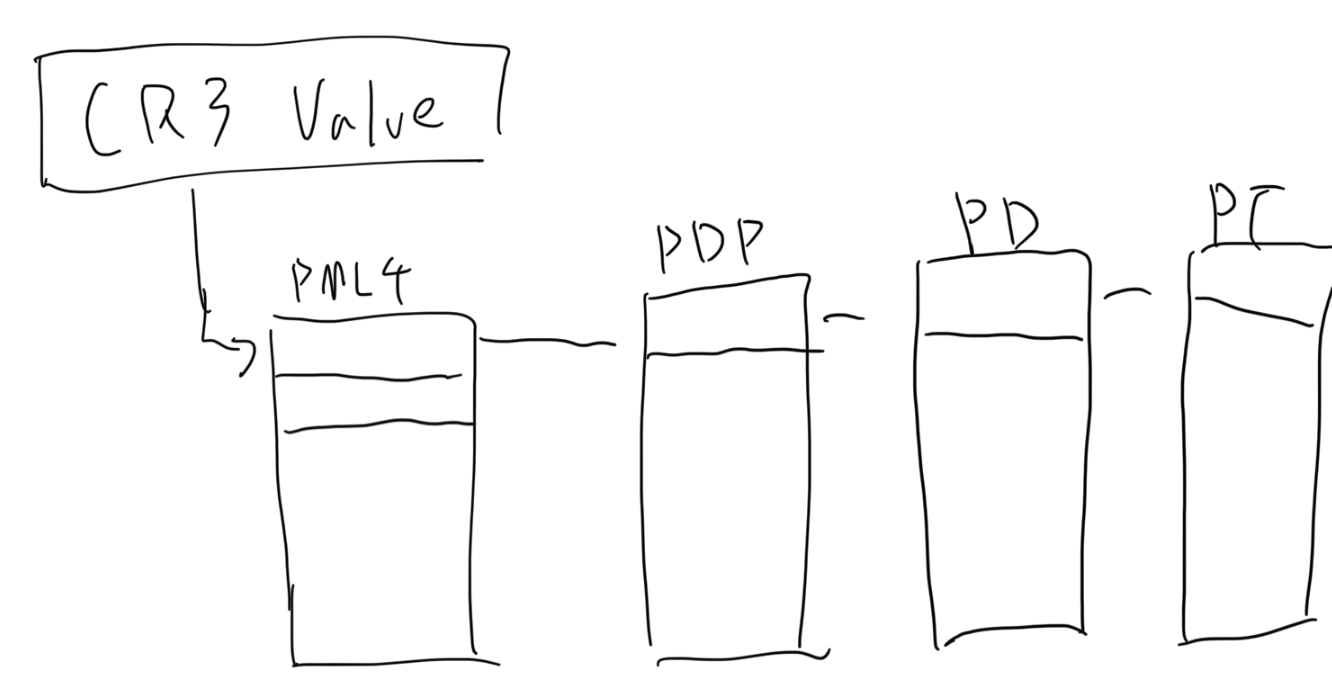
\includegraphics[bb=0 0 1000 360,width=15cm]{img/tegaki/paging.png}
    \end{center}
\end{figure}

\section{本研究で保持する情報}
\label{section:info}

これまでで述べたように,本研究では,メモリダンプを局所的に取得し,動作中のコンピュータのメモリを探索することで,ネットワーク越しにある物理的なコンピュータからオペレーティングシステムのコンテキストを復元することを目的と設定した.
そこで,本研究では,事前に解析者が保持する情報として,監視対象ホストのオペレーティングシステムの種類とバージョン情報を与えるものとする.

\section{なければらならない情報}
\label{section:want}

オペレーティングシステムの状態を保持しているものとして,\ref{section:context}で述べたようにレジスタがある.
しかし,\ref{section:info}で述べたように,現在のレジスタの値など,オペレーティングシステムの状態を保持する領域は,メモリから知ることはできない.
そのため,オペレーティングシステムの内部のシンボル,一例として,プロセス情報を保持するシンボルおよびその型情報を復元することを試みる.
